\documentclass[a4paper, 11pt]{article}
\usepackage{lipsum} %This package just generates Lorem Ipsum filler text. 
\usepackage{fullpage} % changes the margin
\usepackage{mathpazo}
\usepackage{multicol}
\usepackage{graphicx}
\usepackage{enumerate}
\usepackage{amsmath,amsfonts,amsthm} % Math packages
\usepackage{listings}
\usepackage{matlab-prettifier}

\begin{document}
%Header-Make sure you update this information!!!!
\noindent
\large\textbf{Homework 7} \hfill \textbf{Hongyu Yan (516030910595)} \\
\normalsize {\bf CS 259 Numerical Methods for Data Science} \hfill ACM Class, Zhiyuan College, SJTU\\
Prof.~{\bf David Bindel} \hfill Due Date: July 2, 2018\\
TA.~{\bf Yurong You, Xinran Zhu} \hfill Submit Date: \today

\section*{Problem 1}
$X = [x_1, x_2, \cdots, x_n]$. In order to minimize $\|Ac-f_X\|^2$,
we have $c=A^{\dagger}f_X$. In this problem, we have $\mathcal{A}[f_X]=T(x)^TA^{\dagger}f_X$, where $T(x) = \begin{bmatrix}
T_0(x) \\
T_1(x) \\
\vdots \\
T_{n-1}(x)
\end{bmatrix}$, so:
\begin{align*}
& \|\mathcal{A}[f_X+u]-\mathcal{A}[f_X]\|_{\infty} \\
= &\|T(x)^TA^{\dagger}(f_X+u-f_X)\|_{\infty} \\
\leq & \| T(x)^T\|_{\infty}\|A^{\dagger}\|_{\infty}\|u\|_{\infty}
\end{align*}
When $x \in [-1,1]$, $T(x) \leq 1$, then $\|T(x)^T\|_{\infty} \leq n$. So $\| \mathcal{A}[f_X+u]-\mathcal{A}[f_X]\|_{\infty} \leq n\|A^{\dagger}\|_{\infty}\|u\|_{\infty}$, which means $L \leq n\|A^{\dagger}\|_{\infty}$


Here is my MATLAB code for ploting relationship between $n\|A^{\dagger}\|_{\infty}$ versus n.
\begin{lstlisting}[language = Matlab, numbers=left,   
  numberstyle=\tiny,keywordstyle=\color{blue!70},  
  commentstyle=\color{red!50!green!50!blue!50},frame=shadowbox,  
  rulesepcolor=\color{red!20!green!20!blue!20},basicstyle=\ttfamily,
  tabsize=2]
X = zeros(3,1);
Y = zeros(3,1);
m = 7;
for k = 1:3
	n = k*m;
	x = linspace(-1, 1, n);
	A = chebmatrix(x, n);
	X(k) = n;
	Y(k) = n * norm(pinv(A), inf);
end
semilogy(X, Y, '--o');
xlabel('n');
ylabel('n||A||_{\infty}');
\end{lstlisting}
The plot is as below, which is approximately a straight line:
\begin{figure}[htbp]
\centering
	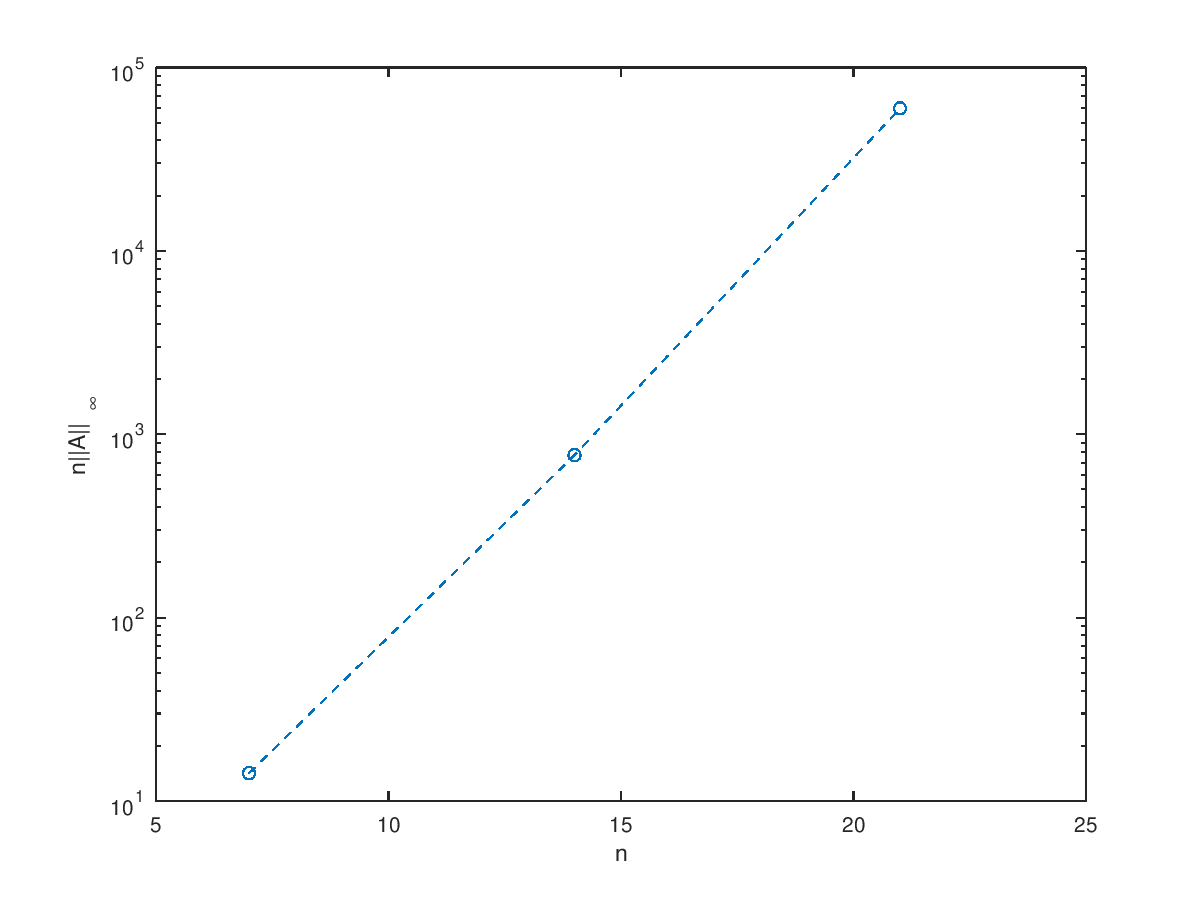
\includegraphics[scale=0.6]{figure/p1.png}
	\caption{$n\|A^{\dagger}\|_{\infty}$ versus n(m=7)}
	\label{fig1}
\end{figure}

\newpage
\section*{Problem 2}
My code is as below:
\begin{lstlisting}[language = Matlab, numbers=left,   
  numberstyle=\tiny,keywordstyle=\color{blue!70},  
  commentstyle=\color{red!50!green!50!blue!50},frame=shadowbox,  
  rulesepcolor=\color{red!20!green!20!blue!20},basicstyle=\ttfamily,
  tabsize=2]
x = linspace(-1, 1, 10);
fx = sin(2 * pi * x);

% generate Kxx, P
Kxx = zeros(10, 10);
for i = 1:10
	for j = 1:10
		Kxx(i,j) = abs((x(i)-x(j))^3);
	end
end
P = [ones(10, 1) x'];

A = [Kxx, P; P' zeros(2, 2)];
b = [fx'; zeros(2, 1)];
tmp = A\b;

d1 = tmp(11);
d2 = tmp(12);
% f(x) = d1 + d2*x + sum(c_i*|x_i-x_j|^3)

x_fit = linspace(-1, 1, 100);
y = f(tmp, x_fit);
y_true = sin(2 * pi * x_fit);

figure(1);
plot(x_fit, y, x_fit, y_true);
xlabel('x');
ylabel('y');
legend('interpolation curve', 'ground truth');

figure(2);
plot(x_fit, (y - y_true).^2);
xlabel('x');
ylabel('approximation error');
\end{lstlisting}
\begin{lstlisting}[language = Matlab, numbers=left,   
  numberstyle=\tiny,keywordstyle=\color{blue!70},  
  commentstyle=\color{red!50!green!50!blue!50},frame=shadowbox,  
  rulesepcolor=\color{red!20!green!20!blue!20},basicstyle=\ttfamily,
  tabsize=2]
function [y] = f(tmp, X)
	x = linspace(-1, 1, 10);
	y = tmp(11) * ones(1, length(X)) + tmp(12) * X;
	for i = 1:10
		y = y + tmp(i) * (abs(X - x(i)).^3);
	end
	  
\end{lstlisting}
\begin{figure}[htbp]
\centering
	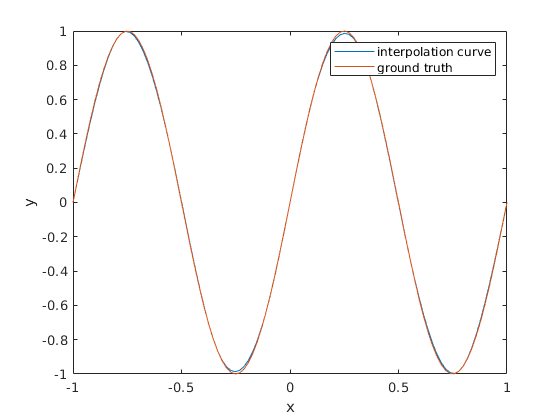
\includegraphics[scale=1.0]{figure/p2_1.png}
	\caption{spline interpolation}
	\label{fig2_1}
\end{figure}

\begin{figure}[htbp]
\centering
	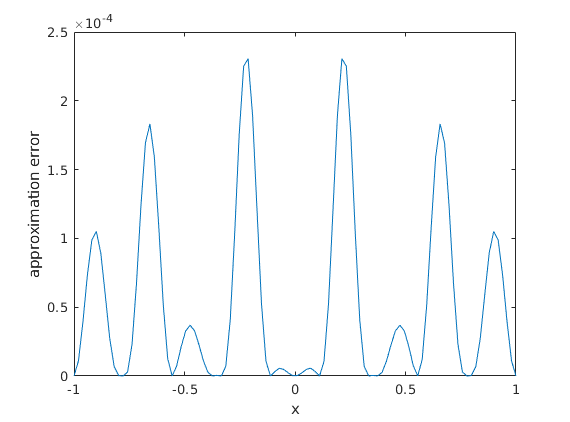
\includegraphics[scale=1.0]{figure/p2_2.png}
	\caption{approximation error}
	\label{fig2_2}
\end{figure}

\end{document}
